\documentclass[twoside]{book}

% Packages required by doxygen
\usepackage{calc}
\usepackage{doxygen}
\usepackage{graphicx}
\usepackage[utf8]{inputenc}
\usepackage{makeidx}
\usepackage{multicol}
\usepackage{multirow}
\usepackage{textcomp}
\usepackage[table]{xcolor}

% Font selection
\usepackage[T1]{fontenc}
\usepackage{mathptmx}
\usepackage[scaled=.90]{helvet}
\usepackage{courier}
\usepackage{amssymb}
\usepackage{sectsty}
\renewcommand{\familydefault}{\sfdefault}
\allsectionsfont{%
  \fontseries{bc}\selectfont%
  \color{darkgray}%
}
\renewcommand{\DoxyLabelFont}{%
  \fontseries{bc}\selectfont%
  \color{darkgray}%
}

% Page & text layout
\usepackage{geometry}
\geometry{%
  a4paper,%
  top=2.5cm,%
  bottom=2.5cm,%
  left=2.5cm,%
  right=2.5cm%
}
\tolerance=750
\hfuzz=15pt
\hbadness=750
\setlength{\emergencystretch}{15pt}
\setlength{\parindent}{0cm}
\setlength{\parskip}{0.2cm}
\makeatletter
\renewcommand{\paragraph}{%
  \@startsection{paragraph}{4}{0ex}{-1.0ex}{1.0ex}{%
    \normalfont\normalsize\bfseries\SS@parafont%
  }%
}
\renewcommand{\subparagraph}{%
  \@startsection{subparagraph}{5}{0ex}{-1.0ex}{1.0ex}{%
    \normalfont\normalsize\bfseries\SS@subparafont%
  }%
}
\makeatother

% Headers & footers
\usepackage{fancyhdr}
\pagestyle{fancyplain}
\fancyhead[LE]{\fancyplain{}{\bfseries\thepage}}
\fancyhead[CE]{\fancyplain{}{}}
\fancyhead[RE]{\fancyplain{}{\bfseries\leftmark}}
\fancyhead[LO]{\fancyplain{}{\bfseries\rightmark}}
\fancyhead[CO]{\fancyplain{}{}}
\fancyhead[RO]{\fancyplain{}{\bfseries\thepage}}
\fancyfoot[LE]{\fancyplain{}{}}
\fancyfoot[CE]{\fancyplain{}{}}
\fancyfoot[RE]{\fancyplain{}{\bfseries\scriptsize Generated on Thu Apr 10 2014 23\-:50\-:25 for Snuffbox by Doxygen }}
\fancyfoot[LO]{\fancyplain{}{\bfseries\scriptsize Generated on Thu Apr 10 2014 23\-:50\-:25 for Snuffbox by Doxygen }}
\fancyfoot[CO]{\fancyplain{}{}}
\fancyfoot[RO]{\fancyplain{}{}}
\renewcommand{\footrulewidth}{0.4pt}
\renewcommand{\chaptermark}[1]{%
  \markboth{#1}{}%
}
\renewcommand{\sectionmark}[1]{%
  \markright{\thesection\ #1}%
}

% Indices & bibliography
\usepackage{natbib}
\usepackage[titles]{tocloft}
\setcounter{tocdepth}{3}
\setcounter{secnumdepth}{5}
\makeindex

% Hyperlinks (required, but should be loaded last)
\usepackage{ifpdf}
\ifpdf
  \usepackage[pdftex,pagebackref=true]{hyperref}
\else
  \usepackage[ps2pdf,pagebackref=true]{hyperref}
\fi
\hypersetup{%
  colorlinks=true,%
  linkcolor=blue,%
  citecolor=blue,%
  unicode%
}

% Custom commands
\newcommand{\clearemptydoublepage}{%
  \newpage{\pagestyle{empty}\cleardoublepage}%
}


%===== C O N T E N T S =====

\begin{document}

% Titlepage & ToC
\hypersetup{pageanchor=false}
\pagenumbering{roman}
\begin{titlepage}
\vspace*{7cm}
\begin{center}%
{\Large Snuffbox \\[1ex]\large Alpha }\\
\vspace*{1cm}
{\large Generated by Doxygen 1.8.6}\\
\vspace*{0.5cm}
{\small Thu Apr 10 2014 23:50:25}\\
\end{center}
\end{titlepage}
\clearemptydoublepage
\tableofcontents
\clearemptydoublepage
\pagenumbering{arabic}
\hypersetup{pageanchor=true}

%--- Begin generated contents ---
\chapter{Hierarchical Index}
\section{Class Hierarchy}
This inheritance list is sorted roughly, but not completely, alphabetically\-:\begin{DoxyCompactList}
\item \contentsline{section}{snuffbox\-:\-:Allocated\-Memory}{\pageref{structsnuffbox_1_1_allocated_memory}}{}
\item \contentsline{section}{snuffbox\-:\-:Game}{\pageref{classsnuffbox_1_1_game}}{}
\item \contentsline{section}{snuffbox\-:\-:I\-Platform\-Window}{\pageref{classsnuffbox_1_1_i_platform_window}}{}
\begin{DoxyCompactList}
\item \contentsline{section}{snuffbox\-:\-:Win32\-Window}{\pageref{classsnuffbox_1_1_win32_window}}{}
\end{DoxyCompactList}
\item \contentsline{section}{snuffbox\-:\-:J\-S\-State\-Wrapper}{\pageref{classsnuffbox_1_1_j_s_state_wrapper}}{}
\item \contentsline{section}{snuffbox\-:\-:Platform\-Window\-Params}{\pageref{structsnuffbox_1_1_platform_window_params}}{}
\item \contentsline{section}{snuffbox\-:\-:Ref\-Count$<$ T $>$}{\pageref{classsnuffbox_1_1_ref_count}}{}
\item \contentsline{section}{snuffbox\-:\-:Ref\-Count$<$ Platform\-Window $>$}{\pageref{classsnuffbox_1_1_ref_count}}{}
\item \contentsline{section}{snuffbox\-:\-:Shared\-Ptr$<$ T $>$}{\pageref{classsnuffbox_1_1_shared_ptr}}{}
\item \contentsline{section}{snuffbox\-:\-:Shared\-Ptr$<$ Platform\-Window $>$}{\pageref{classsnuffbox_1_1_shared_ptr}}{}
\end{DoxyCompactList}

\chapter{Class Index}
\section{Class List}
Here are the classes, structs, unions and interfaces with brief descriptions\-:\begin{DoxyCompactList}
\item\contentsline{section}{\hyperlink{structsnuffbox_1_1_allocated_memory}{snuffbox\-::\-Allocated\-Memory} \\*Contains information about the number of allocations and allocated memory, also checks for leaks on destruction }{\pageref{structsnuffbox_1_1_allocated_memory}}{}
\item\contentsline{section}{\hyperlink{classsnuffbox_1_1_game}{snuffbox\-::\-Game} \\*This is where all the magic happens }{\pageref{classsnuffbox_1_1_game}}{}
\item\contentsline{section}{\hyperlink{classsnuffbox_1_1_i_platform_window}{snuffbox\-::\-I\-Platform\-Window} \\*The base class of all platform windows, all methods should be implemented }{\pageref{classsnuffbox_1_1_i_platform_window}}{}
\item\contentsline{section}{\hyperlink{classsnuffbox_1_1_j_s_state_wrapper}{snuffbox\-::\-J\-S\-State\-Wrapper} \\*Wraps the whole Java\-Script state for use throughout the whole application }{\pageref{classsnuffbox_1_1_j_s_state_wrapper}}{}
\item\contentsline{section}{\hyperlink{structsnuffbox_1_1_platform_window_params}{snuffbox\-::\-Platform\-Window\-Params} \\*Contains all parameters a window was created with }{\pageref{structsnuffbox_1_1_platform_window_params}}{}
\item\contentsline{section}{\hyperlink{classsnuffbox_1_1_ref_count}{snuffbox\-::\-Ref\-Count$<$ T $>$} \\*Used for snuffbox\-::\-Shared\-Ptr$<$\-T$>$ to keep its references }{\pageref{classsnuffbox_1_1_ref_count}}{}
\item\contentsline{section}{\hyperlink{classsnuffbox_1_1_shared_ptr}{snuffbox\-::\-Shared\-Ptr$<$ T $>$} \\*A garbage collecting shared pointer, so memory management won't become a worry }{\pageref{classsnuffbox_1_1_shared_ptr}}{}
\item\contentsline{section}{\hyperlink{classsnuffbox_1_1_win32_window}{snuffbox\-::\-Win32\-Window} \\*A Windows window for use with the engine }{\pageref{classsnuffbox_1_1_win32_window}}{}
\end{DoxyCompactList}

\chapter{Class Documentation}
\hypertarget{structsnuffbox_1_1_allocated_memory}{\section{snuffbox\-:\-:Allocated\-Memory Struct Reference}
\label{structsnuffbox_1_1_allocated_memory}\index{snuffbox\-::\-Allocated\-Memory@{snuffbox\-::\-Allocated\-Memory}}
}


Contains information about the number of allocations and allocated memory, also checks for leaks on destruction.  




{\ttfamily \#include $<$allocated\-\_\-memory.\-h$>$}

\subsection*{Public Member Functions}
\begin{DoxyCompactItemize}
\item 
\hypertarget{structsnuffbox_1_1_allocated_memory_a6737b0bf2fc015ecf4fd80e3130d560b}{\hyperlink{structsnuffbox_1_1_allocated_memory_a6737b0bf2fc015ecf4fd80e3130d560b}{Allocated\-Memory} ()}\label{structsnuffbox_1_1_allocated_memory_a6737b0bf2fc015ecf4fd80e3130d560b}

\begin{DoxyCompactList}\small\item\em Default constructor. \end{DoxyCompactList}\item 
\hypertarget{structsnuffbox_1_1_allocated_memory_ad31b0fbc7e06d484c14de7156dd244af}{\hyperlink{structsnuffbox_1_1_allocated_memory_ad31b0fbc7e06d484c14de7156dd244af}{$\sim$\-Allocated\-Memory} ()}\label{structsnuffbox_1_1_allocated_memory_ad31b0fbc7e06d484c14de7156dd244af}

\begin{DoxyCompactList}\small\item\em Default destructor (Checks for leaks) \end{DoxyCompactList}\item 
\hypertarget{structsnuffbox_1_1_allocated_memory_a5445bb11a72374119295b955174ca943}{{\footnotesize template$<$typename T , typename... Args$>$ }\\T $\ast$ \hyperlink{structsnuffbox_1_1_allocated_memory_a5445bb11a72374119295b955174ca943}{Construct\-Shared} (Args \&\&...args)}\label{structsnuffbox_1_1_allocated_memory_a5445bb11a72374119295b955174ca943}

\begin{DoxyCompactList}\small\item\em Constructs a shared pointer. \end{DoxyCompactList}\item 
\hypertarget{structsnuffbox_1_1_allocated_memory_aaf31f5684b58389919ae0c5e314564b5}{{\footnotesize template$<$typename T $>$ }\\void \hyperlink{structsnuffbox_1_1_allocated_memory_aaf31f5684b58389919ae0c5e314564b5}{Destruct} (T $\ast$ptr)}\label{structsnuffbox_1_1_allocated_memory_aaf31f5684b58389919ae0c5e314564b5}

\begin{DoxyCompactList}\small\item\em Destructs a pointer. \end{DoxyCompactList}\end{DoxyCompactItemize}
\subsection*{Public Attributes}
\begin{DoxyCompactItemize}
\item 
\hypertarget{structsnuffbox_1_1_allocated_memory_a548ff93967d1bf9dc435e65501200051}{unsigned int \hyperlink{structsnuffbox_1_1_allocated_memory_a548ff93967d1bf9dc435e65501200051}{allocations}}\label{structsnuffbox_1_1_allocated_memory_a548ff93967d1bf9dc435e65501200051}

\begin{DoxyCompactList}\small\item\em The number of allocations of this allocator. \end{DoxyCompactList}\item 
\hypertarget{structsnuffbox_1_1_allocated_memory_a0950edd703237dd9bc946a82463c2887}{size\-\_\-t \hyperlink{structsnuffbox_1_1_allocated_memory_a0950edd703237dd9bc946a82463c2887}{allocated\-Memory}}\label{structsnuffbox_1_1_allocated_memory_a0950edd703237dd9bc946a82463c2887}

\begin{DoxyCompactList}\small\item\em The total allocated memory in bytes of this allocator. \end{DoxyCompactList}\end{DoxyCompactItemize}


\subsection{Detailed Description}
Contains information about the number of allocations and allocated memory, also checks for leaks on destruction. 

\begin{DoxyAuthor}{Author}
Dani�l Konings 
\end{DoxyAuthor}


The documentation for this struct was generated from the following files\-:\begin{DoxyCompactItemize}
\item 
C\-:/\-Snuff/src/snuffbox/memory/allocated\-\_\-memory.\-h\item 
C\-:/\-Snuff/src/snuffbox/memory/allocated\-\_\-memory.\-cc\end{DoxyCompactItemize}

\hypertarget{classsnuffbox_1_1_game}{\section{snuffbox\-:\-:Game Class Reference}
\label{classsnuffbox_1_1_game}\index{snuffbox\-::\-Game@{snuffbox\-::\-Game}}
}


This is where all the magic happens.  




{\ttfamily \#include $<$game.\-h$>$}

Inheritance diagram for snuffbox\-:\-:Game\-:\begin{figure}[H]
\begin{center}
\leavevmode
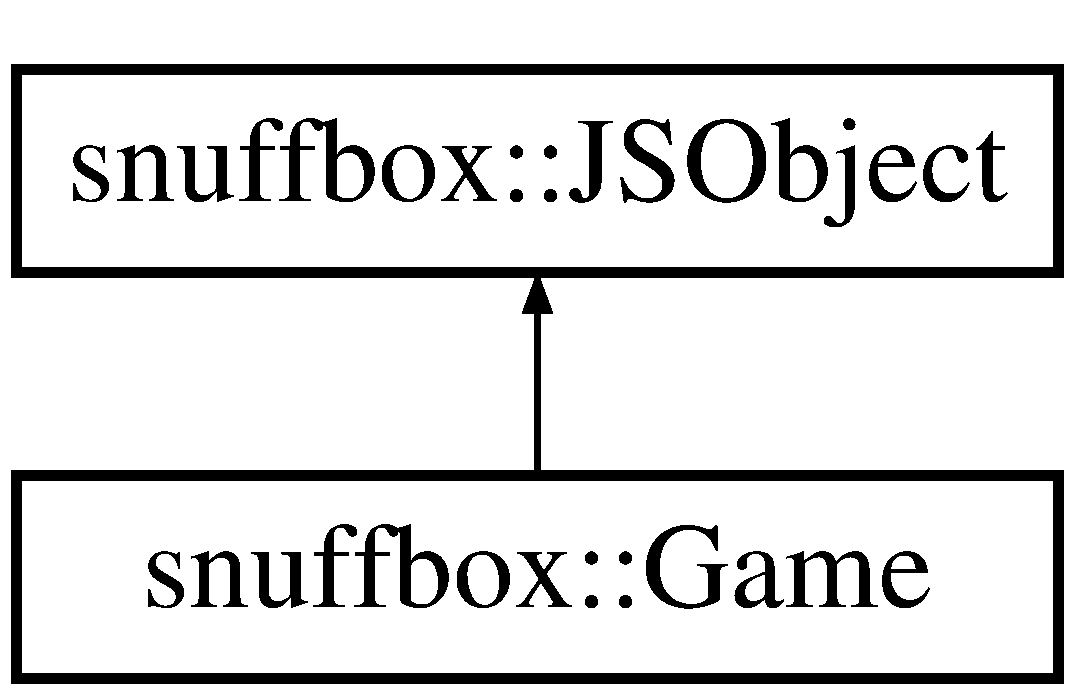
\includegraphics[height=2.000000cm]{classsnuffbox_1_1_game}
\end{center}
\end{figure}
\subsection*{Public Member Functions}
\begin{DoxyCompactItemize}
\item 
\hypertarget{classsnuffbox_1_1_game_ac29903476c91c02c01035feddf9f44bf}{\hyperlink{classsnuffbox_1_1_game_ac29903476c91c02c01035feddf9f44bf}{Game} ()}\label{classsnuffbox_1_1_game_ac29903476c91c02c01035feddf9f44bf}

\begin{DoxyCompactList}\small\item\em Default constructor. \end{DoxyCompactList}\item 
\hypertarget{classsnuffbox_1_1_game_a1e5196dbba1c6a65c8141108b2b93c75}{\hyperlink{classsnuffbox_1_1_game_a1e5196dbba1c6a65c8141108b2b93c75}{Game} (Platform\-Window $\ast$\hyperlink{classsnuffbox_1_1_game_aff19ed260f04e70c8c2a61d271500154}{window})}\label{classsnuffbox_1_1_game_a1e5196dbba1c6a65c8141108b2b93c75}

\begin{DoxyCompactList}\small\item\em Construct with a window. \end{DoxyCompactList}\item 
\hypertarget{classsnuffbox_1_1_game_ae3d112ca6e0e55150d2fdbc704474530}{\hyperlink{classsnuffbox_1_1_game_ae3d112ca6e0e55150d2fdbc704474530}{$\sim$\-Game} ()}\label{classsnuffbox_1_1_game_ae3d112ca6e0e55150d2fdbc704474530}

\begin{DoxyCompactList}\small\item\em Default destructor. \end{DoxyCompactList}\item 
\hypertarget{classsnuffbox_1_1_game_a26bd9839136e8b541199bf94ef723070}{void \hyperlink{classsnuffbox_1_1_game_a26bd9839136e8b541199bf94ef723070}{Parse\-Command\-Line} ()}\label{classsnuffbox_1_1_game_a26bd9839136e8b541199bf94ef723070}

\begin{DoxyCompactList}\small\item\em Parses the command line. \end{DoxyCompactList}\item 
\hypertarget{classsnuffbox_1_1_game_aef12e15d690ef593ff7c01cee5b6ae74}{std\-::string \hyperlink{classsnuffbox_1_1_game_aef12e15d690ef593ff7c01cee5b6ae74}{Get\-Command} (const std\-::string \&cmd\-Line, const char $\ast$option)}\label{classsnuffbox_1_1_game_aef12e15d690ef593ff7c01cee5b6ae74}

\begin{DoxyCompactList}\small\item\em Finds a command. \end{DoxyCompactList}\item 
\hypertarget{classsnuffbox_1_1_game_a9d913921e1cbb2b2f5fe13e73208de6c}{bool \hyperlink{classsnuffbox_1_1_game_a9d913921e1cbb2b2f5fe13e73208de6c}{Command\-Exists} (const std\-::string \&cmd\-Line, const char $\ast$option)}\label{classsnuffbox_1_1_game_a9d913921e1cbb2b2f5fe13e73208de6c}

\begin{DoxyCompactList}\small\item\em Checks if a command exists. \end{DoxyCompactList}\item 
\hypertarget{classsnuffbox_1_1_game_a1c5373c68261c54aff03e6abe40fee52}{void \hyperlink{classsnuffbox_1_1_game_a1c5373c68261c54aff03e6abe40fee52}{Update} ()}\label{classsnuffbox_1_1_game_a1c5373c68261c54aff03e6abe40fee52}

\begin{DoxyCompactList}\small\item\em Updates the game. \end{DoxyCompactList}\item 
\hypertarget{classsnuffbox_1_1_game_ad3b88fb61f44dbaaf88881cd77590958}{void \hyperlink{classsnuffbox_1_1_game_ad3b88fb61f44dbaaf88881cd77590958}{Shutdown} ()}\label{classsnuffbox_1_1_game_ad3b88fb61f44dbaaf88881cd77590958}

\begin{DoxyCompactList}\small\item\em Shuts the game down. \end{DoxyCompactList}\item 
\hypertarget{classsnuffbox_1_1_game_aff19ed260f04e70c8c2a61d271500154}{Platform\-Window $\ast$ \hyperlink{classsnuffbox_1_1_game_aff19ed260f04e70c8c2a61d271500154}{window} ()}\label{classsnuffbox_1_1_game_aff19ed260f04e70c8c2a61d271500154}

\begin{DoxyCompactList}\small\item\em Returns the window the game is running in. \end{DoxyCompactList}\item 
\hypertarget{classsnuffbox_1_1_game_ae1ace018b9c60591d02d34b575e67f37}{bool \hyperlink{classsnuffbox_1_1_game_ae1ace018b9c60591d02d34b575e67f37}{started} ()}\label{classsnuffbox_1_1_game_ae1ace018b9c60591d02d34b575e67f37}

\begin{DoxyCompactList}\small\item\em Returns if the game is started or not. \end{DoxyCompactList}\item 
\hypertarget{classsnuffbox_1_1_game_a36ec7d7e374dfed1acd2547f2f60e7ba}{void \hyperlink{classsnuffbox_1_1_game_a36ec7d7e374dfed1acd2547f2f60e7ba}{Notify\-Event} (Game\-Events evt)}\label{classsnuffbox_1_1_game_a36ec7d7e374dfed1acd2547f2f60e7ba}

\begin{DoxyCompactList}\small\item\em Notify the game of an event. \end{DoxyCompactList}\item 
\hypertarget{classsnuffbox_1_1_game_a2691166254d3fc52ac1cf7feb1a2902b}{void \hyperlink{classsnuffbox_1_1_game_a2691166254d3fc52ac1cf7feb1a2902b}{Initialise\-Window} ()}\label{classsnuffbox_1_1_game_a2691166254d3fc52ac1cf7feb1a2902b}

\begin{DoxyCompactList}\small\item\em Initialises, creates and shows the window. \end{DoxyCompactList}\item 
\hypertarget{classsnuffbox_1_1_game_ac930fcb620166ae25ecd283e69a27fd1}{void \hyperlink{classsnuffbox_1_1_game_ac930fcb620166ae25ecd283e69a27fd1}{Create\-Callbacks} ()}\label{classsnuffbox_1_1_game_ac930fcb620166ae25ecd283e69a27fd1}

\begin{DoxyCompactList}\small\item\em Creates the Java\-Script callbacks. \end{DoxyCompactList}\item 
\hypertarget{classsnuffbox_1_1_game_a19d726a070d51db1a22d3db2bed3a033}{\hyperlink{classsnuffbox_1_1_game_a19d726a070d51db1a22d3db2bed3a033}{J\-S\-\_\-\-N\-A\-M\-E} (\hyperlink{classsnuffbox_1_1_game}{Game})}\label{classsnuffbox_1_1_game_a19d726a070d51db1a22d3db2bed3a033}

\begin{DoxyCompactList}\small\item\em The Java\-Script update callback. \end{DoxyCompactList}\end{DoxyCompactItemize}
\subsection*{Static Public Member Functions}
\begin{DoxyCompactItemize}
\item 
\hypertarget{classsnuffbox_1_1_game_abfb0a8d3e56cf9450527fbd7990a22e8}{static void \hyperlink{classsnuffbox_1_1_game_abfb0a8d3e56cf9450527fbd7990a22e8}{Register\-J\-S} (J\-S\-\_\-\-T\-E\-M\-P\-L\-A\-T\-E)}\label{classsnuffbox_1_1_game_abfb0a8d3e56cf9450527fbd7990a22e8}

\begin{DoxyCompactList}\small\item\em Registers all Java\-Script functions. \end{DoxyCompactList}\end{DoxyCompactItemize}


\subsection{Detailed Description}
This is where all the magic happens. 

\begin{DoxyAuthor}{Author}
Dani�l Konings 
\end{DoxyAuthor}


The documentation for this class was generated from the following files\-:\begin{DoxyCompactItemize}
\item 
C\-:/\-Snuff/src/snuffbox/game.\-h\item 
C\-:/\-Snuff/src/snuffbox/game.\-cc\end{DoxyCompactItemize}

\hypertarget{classsnuffbox_1_1_i_platform_window}{\section{snuffbox\-:\-:I\-Platform\-Window Class Reference}
\label{classsnuffbox_1_1_i_platform_window}\index{snuffbox\-::\-I\-Platform\-Window@{snuffbox\-::\-I\-Platform\-Window}}
}


The base class of all platform windows, all methods should be implemented.  




{\ttfamily \#include $<$interfaces.\-h$>$}

Inheritance diagram for snuffbox\-:\-:I\-Platform\-Window\-:\begin{figure}[H]
\begin{center}
\leavevmode
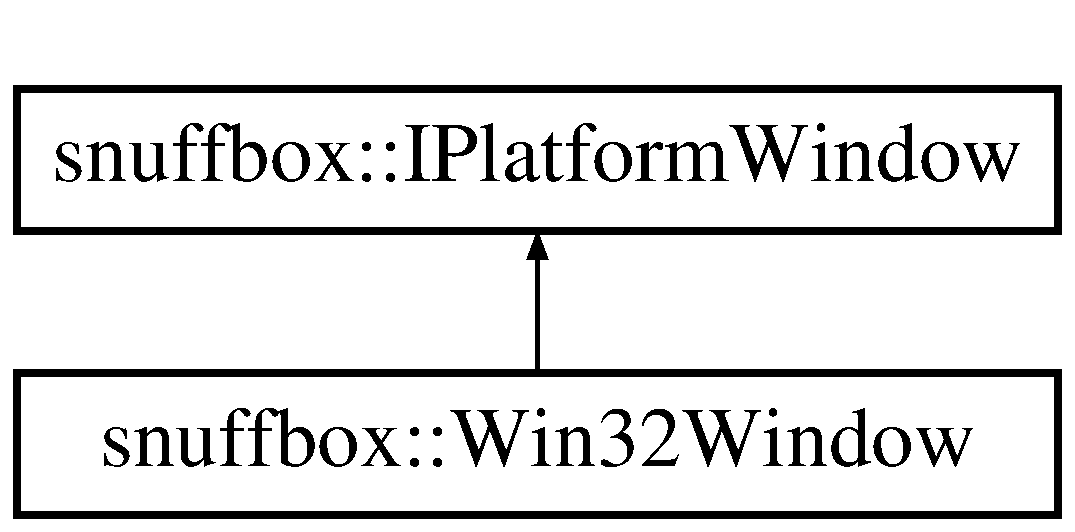
\includegraphics[height=2.000000cm]{classsnuffbox_1_1_i_platform_window}
\end{center}
\end{figure}
\subsection*{Public Member Functions}
\begin{DoxyCompactItemize}
\item 
\hypertarget{classsnuffbox_1_1_i_platform_window_a89ee9662088f169639e37551682a48ea}{virtual void \hyperlink{classsnuffbox_1_1_i_platform_window_a89ee9662088f169639e37551682a48ea}{Create} ()=0}\label{classsnuffbox_1_1_i_platform_window_a89ee9662088f169639e37551682a48ea}

\begin{DoxyCompactList}\small\item\em Creates the window. \end{DoxyCompactList}\item 
\hypertarget{classsnuffbox_1_1_i_platform_window_a8572749f1909c64faa17492f8fe988d4}{virtual void \hyperlink{classsnuffbox_1_1_i_platform_window_a8572749f1909c64faa17492f8fe988d4}{Show} ()=0}\label{classsnuffbox_1_1_i_platform_window_a8572749f1909c64faa17492f8fe988d4}

\begin{DoxyCompactList}\small\item\em Shows the window. \end{DoxyCompactList}\item 
\hypertarget{classsnuffbox_1_1_i_platform_window_aa78df06769fcc169559f18d5b87d7126}{virtual void \hyperlink{classsnuffbox_1_1_i_platform_window_aa78df06769fcc169559f18d5b87d7126}{Destroy} ()=0}\label{classsnuffbox_1_1_i_platform_window_aa78df06769fcc169559f18d5b87d7126}

\begin{DoxyCompactList}\small\item\em Destroys the window. \end{DoxyCompactList}\item 
\hypertarget{classsnuffbox_1_1_i_platform_window_abee93eb43c3308ef7025e69ac09b5e74}{virtual void \hyperlink{classsnuffbox_1_1_i_platform_window_abee93eb43c3308ef7025e69ac09b5e74}{On\-Set\-Focus} ()=0}\label{classsnuffbox_1_1_i_platform_window_abee93eb43c3308ef7025e69ac09b5e74}

\begin{DoxyCompactList}\small\item\em When the window is focussed. \end{DoxyCompactList}\item 
\hypertarget{classsnuffbox_1_1_i_platform_window_ac0039729097c326102b86e313356c75f}{virtual void \hyperlink{classsnuffbox_1_1_i_platform_window_ac0039729097c326102b86e313356c75f}{On\-Kill\-Focus} ()=0}\label{classsnuffbox_1_1_i_platform_window_ac0039729097c326102b86e313356c75f}

\begin{DoxyCompactList}\small\item\em When the window focus is killed. \end{DoxyCompactList}\item 
\hypertarget{classsnuffbox_1_1_i_platform_window_a80bafb8f6d5fbba4b4dbce33546fe241}{virtual void \hyperlink{classsnuffbox_1_1_i_platform_window_a80bafb8f6d5fbba4b4dbce33546fe241}{On\-Close} ()=0}\label{classsnuffbox_1_1_i_platform_window_a80bafb8f6d5fbba4b4dbce33546fe241}

\begin{DoxyCompactList}\small\item\em When the window is closed. \end{DoxyCompactList}\item 
\hypertarget{classsnuffbox_1_1_i_platform_window_a3ca2312a6671a9daba251b3e0976a5b5}{virtual void \hyperlink{classsnuffbox_1_1_i_platform_window_a3ca2312a6671a9daba251b3e0976a5b5}{Process\-Messages} ()=0}\label{classsnuffbox_1_1_i_platform_window_a3ca2312a6671a9daba251b3e0976a5b5}

\begin{DoxyCompactList}\small\item\em Processes all messages. \end{DoxyCompactList}\item 
\hypertarget{classsnuffbox_1_1_i_platform_window_adedbb774b7b37552c738475837ae7323}{\hyperlink{structsnuffbox_1_1_platform_window_params}{Platform\-Window\-Params} \& \hyperlink{classsnuffbox_1_1_i_platform_window_adedbb774b7b37552c738475837ae7323}{params} ()}\label{classsnuffbox_1_1_i_platform_window_adedbb774b7b37552c738475837ae7323}

\begin{DoxyCompactList}\small\item\em Returns the parameters structure of this window. \end{DoxyCompactList}\end{DoxyCompactItemize}


\subsection{Detailed Description}
The base class of all platform windows, all methods should be implemented. 

\begin{DoxyAuthor}{Author}
Dani�l Konings 
\end{DoxyAuthor}


The documentation for this class was generated from the following file\-:\begin{DoxyCompactItemize}
\item 
C\-:/\-Snuff/src/snuffbox/platform/interfaces.\-h\end{DoxyCompactItemize}

\hypertarget{structsnuffbox_1_1_platform_window_params}{\section{snuffbox\-:\-:Platform\-Window\-Params Struct Reference}
\label{structsnuffbox_1_1_platform_window_params}\index{snuffbox\-::\-Platform\-Window\-Params@{snuffbox\-::\-Platform\-Window\-Params}}
}


Contains all parameters a window was created with.  




{\ttfamily \#include $<$interfaces.\-h$>$}

\subsection*{Public Attributes}
\begin{DoxyCompactItemize}
\item 
\hypertarget{structsnuffbox_1_1_platform_window_params_acdb39d6191fc486fe5b6da1d83a426c0}{int {\bfseries x}}\label{structsnuffbox_1_1_platform_window_params_acdb39d6191fc486fe5b6da1d83a426c0}

\item 
\hypertarget{structsnuffbox_1_1_platform_window_params_ae0b46b315d567755b5bc1baec2f401be}{int {\bfseries y}}\label{structsnuffbox_1_1_platform_window_params_ae0b46b315d567755b5bc1baec2f401be}

\item 
\hypertarget{structsnuffbox_1_1_platform_window_params_a41bd34e7a5718eb3d09605f2063ce200}{int {\bfseries w}}\label{structsnuffbox_1_1_platform_window_params_a41bd34e7a5718eb3d09605f2063ce200}

\item 
\hypertarget{structsnuffbox_1_1_platform_window_params_a01272a40a98233f040f0d3a402f4e558}{int {\bfseries h}}\label{structsnuffbox_1_1_platform_window_params_a01272a40a98233f040f0d3a402f4e558}

\item 
\hypertarget{structsnuffbox_1_1_platform_window_params_abeebd3b9c4f62afe4ac2bae30390599c}{const char $\ast$ {\bfseries name}}\label{structsnuffbox_1_1_platform_window_params_abeebd3b9c4f62afe4ac2bae30390599c}

\end{DoxyCompactItemize}


\subsection{Detailed Description}
Contains all parameters a window was created with. 

\begin{DoxyAuthor}{Author}
Dani�l Konings 
\end{DoxyAuthor}


The documentation for this struct was generated from the following file\-:\begin{DoxyCompactItemize}
\item 
C\-:/\-Snuff/src/snuffbox/platform/interfaces.\-h\end{DoxyCompactItemize}

\hypertarget{classsnuffbox_1_1_ref_count}{\section{snuffbox\-:\-:Ref\-Count$<$ T $>$ Class Template Reference}
\label{classsnuffbox_1_1_ref_count}\index{snuffbox\-::\-Ref\-Count$<$ T $>$@{snuffbox\-::\-Ref\-Count$<$ T $>$}}
}


Used for snuffbox\-::\-Shared\-Ptr$<$\-T$>$ to keep its references.  




{\ttfamily \#include $<$shared\-\_\-ptr.\-h$>$}

\subsection*{Public Member Functions}
\begin{DoxyCompactItemize}
\item 
\hypertarget{classsnuffbox_1_1_ref_count_a47d8b6e14dd15ae6301f2728517e743c}{\hyperlink{classsnuffbox_1_1_ref_count_a47d8b6e14dd15ae6301f2728517e743c}{Ref\-Count} ()}\label{classsnuffbox_1_1_ref_count_a47d8b6e14dd15ae6301f2728517e743c}

\begin{DoxyCompactList}\small\item\em Default constructor. \end{DoxyCompactList}\item 
\hypertarget{classsnuffbox_1_1_ref_count_ae3d059a44d0fa179576f7953e8927f67}{\hyperlink{classsnuffbox_1_1_ref_count_ae3d059a44d0fa179576f7953e8927f67}{Ref\-Count} (T $\ast$ptr)}\label{classsnuffbox_1_1_ref_count_ae3d059a44d0fa179576f7953e8927f67}

\begin{DoxyCompactList}\small\item\em Construction through pointer. \end{DoxyCompactList}\item 
\hypertarget{classsnuffbox_1_1_ref_count_a29a8fa7fdf3faf256bdf535d01434a16}{\hyperlink{classsnuffbox_1_1_ref_count_a29a8fa7fdf3faf256bdf535d01434a16}{$\sim$\-Ref\-Count} ()}\label{classsnuffbox_1_1_ref_count_a29a8fa7fdf3faf256bdf535d01434a16}

\begin{DoxyCompactList}\small\item\em Default destructor. \end{DoxyCompactList}\item 
\hypertarget{classsnuffbox_1_1_ref_count_a5777549d4caba3f225fe1c4bc50ac4df}{void \hyperlink{classsnuffbox_1_1_ref_count_a5777549d4caba3f225fe1c4bc50ac4df}{Destroy} ()}\label{classsnuffbox_1_1_ref_count_a5777549d4caba3f225fe1c4bc50ac4df}

\begin{DoxyCompactList}\small\item\em Destroys the associated pointer. \end{DoxyCompactList}\item 
\hypertarget{classsnuffbox_1_1_ref_count_aab459934009e01d2859ae364098f8c80}{void \hyperlink{classsnuffbox_1_1_ref_count_aab459934009e01d2859ae364098f8c80}{Increase\-Ref} ()}\label{classsnuffbox_1_1_ref_count_aab459934009e01d2859ae364098f8c80}

\begin{DoxyCompactList}\small\item\em Increases the reference count by one. \end{DoxyCompactList}\item 
\hypertarget{classsnuffbox_1_1_ref_count_a5c21383e14e7d71424a6982a47f9d2b7}{void \hyperlink{classsnuffbox_1_1_ref_count_a5c21383e14e7d71424a6982a47f9d2b7}{Decrease\-Ref} ()}\label{classsnuffbox_1_1_ref_count_a5c21383e14e7d71424a6982a47f9d2b7}

\begin{DoxyCompactList}\small\item\em Decreases the reference count by one. \end{DoxyCompactList}\end{DoxyCompactItemize}


\subsection{Detailed Description}
\subsubsection*{template$<$typename T$>$class snuffbox\-::\-Ref\-Count$<$ T $>$}

Used for snuffbox\-::\-Shared\-Ptr$<$\-T$>$ to keep its references. 

\begin{DoxyAuthor}{Author}
Dani�l Konings 
\end{DoxyAuthor}


The documentation for this class was generated from the following file\-:\begin{DoxyCompactItemize}
\item 
C\-:/\-Snuff/src/snuffbox/memory/shared\-\_\-ptr.\-h\end{DoxyCompactItemize}

\hypertarget{classsnuffbox_1_1_shared_ptr}{\section{snuffbox\-:\-:Shared\-Ptr$<$ T $>$ Class Template Reference}
\label{classsnuffbox_1_1_shared_ptr}\index{snuffbox\-::\-Shared\-Ptr$<$ T $>$@{snuffbox\-::\-Shared\-Ptr$<$ T $>$}}
}
\subsection*{Public Member Functions}
\begin{DoxyCompactItemize}
\item 
\hypertarget{classsnuffbox_1_1_shared_ptr_ab1de15b7502bcad3bd9c7bf82a2a98e7}{\hyperlink{classsnuffbox_1_1_shared_ptr_ab1de15b7502bcad3bd9c7bf82a2a98e7}{Shared\-Ptr} ()}\label{classsnuffbox_1_1_shared_ptr_ab1de15b7502bcad3bd9c7bf82a2a98e7}

\begin{DoxyCompactList}\small\item\em Default constructor. \end{DoxyCompactList}\item 
\hypertarget{classsnuffbox_1_1_shared_ptr_a9b286960622fc23a06f6e2e8b2ed8663}{\hyperlink{classsnuffbox_1_1_shared_ptr_a9b286960622fc23a06f6e2e8b2ed8663}{Shared\-Ptr} (T $\ast$ptr)}\label{classsnuffbox_1_1_shared_ptr_a9b286960622fc23a06f6e2e8b2ed8663}

\begin{DoxyCompactList}\small\item\em Initialisation constructor. \end{DoxyCompactList}\item 
\hypertarget{classsnuffbox_1_1_shared_ptr_a521e70c28535569af7fbe115dd889ccd}{{\bfseries Shared\-Ptr} (const \hyperlink{classsnuffbox_1_1_shared_ptr}{Shared\-Ptr}$<$ T $>$ \&other)}\label{classsnuffbox_1_1_shared_ptr_a521e70c28535569af7fbe115dd889ccd}

\item 
\hypertarget{classsnuffbox_1_1_shared_ptr_a00f79a79261083ccd63d4b57e2046417}{{\bfseries Shared\-Ptr} (\hyperlink{classsnuffbox_1_1_shared_ptr}{Shared\-Ptr}$<$ T $>$ \&\&other)}\label{classsnuffbox_1_1_shared_ptr_a00f79a79261083ccd63d4b57e2046417}

\item 
\hypertarget{classsnuffbox_1_1_shared_ptr_ad8940a1b8cb67b76d5a626dbab64a04d}{\hyperlink{classsnuffbox_1_1_shared_ptr_ad8940a1b8cb67b76d5a626dbab64a04d}{$\sim$\-Shared\-Ptr} ()}\label{classsnuffbox_1_1_shared_ptr_ad8940a1b8cb67b76d5a626dbab64a04d}

\begin{DoxyCompactList}\small\item\em Default destructor. \end{DoxyCompactList}\item 
\hypertarget{classsnuffbox_1_1_shared_ptr_a9961287bcae6ca51a38b2b562e7e3be6}{\hyperlink{classsnuffbox_1_1_shared_ptr}{Shared\-Ptr} \& {\bfseries operator=} (const \hyperlink{classsnuffbox_1_1_shared_ptr}{Shared\-Ptr} \&other)}\label{classsnuffbox_1_1_shared_ptr_a9961287bcae6ca51a38b2b562e7e3be6}

\item 
\hypertarget{classsnuffbox_1_1_shared_ptr_ad840a9a7a7b36a457dac8d65bf1d5302}{\hyperlink{classsnuffbox_1_1_shared_ptr}{Shared\-Ptr} \& {\bfseries operator=} (\hyperlink{classsnuffbox_1_1_shared_ptr}{Shared\-Ptr} \&\&other)}\label{classsnuffbox_1_1_shared_ptr_ad840a9a7a7b36a457dac8d65bf1d5302}

\item 
\hypertarget{classsnuffbox_1_1_shared_ptr_a29e7a5e52d8c5e74d28adc28ff9a6e3b}{T $\ast$ {\bfseries operator-\/$>$} (void)}\label{classsnuffbox_1_1_shared_ptr_a29e7a5e52d8c5e74d28adc28ff9a6e3b}

\item 
\hypertarget{classsnuffbox_1_1_shared_ptr_ababc077f3967c39d36db1d2f06831602}{T \& {\bfseries operator$\ast$} (void)}\label{classsnuffbox_1_1_shared_ptr_ababc077f3967c39d36db1d2f06831602}

\item 
\hypertarget{classsnuffbox_1_1_shared_ptr_a4aada4171efd1890571faf8e08f0a6e5}{bool {\bfseries operator==} (const \hyperlink{classsnuffbox_1_1_shared_ptr}{Shared\-Ptr}$<$ T $>$ \&other) const }\label{classsnuffbox_1_1_shared_ptr_a4aada4171efd1890571faf8e08f0a6e5}

\item 
\hypertarget{classsnuffbox_1_1_shared_ptr_a8adc462fb2c53162745e735658bbc621}{bool {\bfseries operator==} (const T $\ast$other) const }\label{classsnuffbox_1_1_shared_ptr_a8adc462fb2c53162745e735658bbc621}

\item 
\hypertarget{classsnuffbox_1_1_shared_ptr_ad52060b9d84ceed978c8ad158c533188}{bool {\bfseries operator==} (std\-::nullptr\-\_\-t) const }\label{classsnuffbox_1_1_shared_ptr_ad52060b9d84ceed978c8ad158c533188}

\item 
\hypertarget{classsnuffbox_1_1_shared_ptr_a82b1278cc41e288eee3ac78f3ea8c155}{bool {\bfseries operator!=} (const \hyperlink{classsnuffbox_1_1_shared_ptr}{Shared\-Ptr}$<$ T $>$ \&other) const }\label{classsnuffbox_1_1_shared_ptr_a82b1278cc41e288eee3ac78f3ea8c155}

\item 
\hypertarget{classsnuffbox_1_1_shared_ptr_a5f3f696a43b8b584fe8599c5bde49885}{bool {\bfseries operator!=} (const T $\ast$other) const }\label{classsnuffbox_1_1_shared_ptr_a5f3f696a43b8b584fe8599c5bde49885}

\item 
\hypertarget{classsnuffbox_1_1_shared_ptr_aac9f37b77fec92a57a345f8fec07bd01}{bool {\bfseries operator!=} (std\-::nullptr\-\_\-t) const }\label{classsnuffbox_1_1_shared_ptr_aac9f37b77fec92a57a345f8fec07bd01}

\item 
\hypertarget{classsnuffbox_1_1_shared_ptr_a1e6b8170c9151ad4113f98b4e5e86b3d}{void \hyperlink{classsnuffbox_1_1_shared_ptr_a1e6b8170c9151ad4113f98b4e5e86b3d}{Swap} (\hyperlink{classsnuffbox_1_1_shared_ptr}{Shared\-Ptr}$<$ T $>$ \&right)}\label{classsnuffbox_1_1_shared_ptr_a1e6b8170c9151ad4113f98b4e5e86b3d}

\begin{DoxyCompactList}\small\item\em Swaps two Shared\-Ptrs. \end{DoxyCompactList}\item 
\hypertarget{classsnuffbox_1_1_shared_ptr_afa6eb6fd99d2b3e9142573024afc83fc}{void \hyperlink{classsnuffbox_1_1_shared_ptr_afa6eb6fd99d2b3e9142573024afc83fc}{Reset} ()}\label{classsnuffbox_1_1_shared_ptr_afa6eb6fd99d2b3e9142573024afc83fc}

\begin{DoxyCompactList}\small\item\em Resets the shared pointer. \end{DoxyCompactList}\item 
\hypertarget{classsnuffbox_1_1_shared_ptr_ae9748e1ebd5e34e2e184e621816d8497}{void \hyperlink{classsnuffbox_1_1_shared_ptr_ae9748e1ebd5e34e2e184e621816d8497}{Reset} (T $\ast$ptr, \hyperlink{classsnuffbox_1_1_ref_count}{Ref\-Count}$<$ T $>$ $\ast$ref)}\label{classsnuffbox_1_1_shared_ptr_ae9748e1ebd5e34e2e184e621816d8497}

\begin{DoxyCompactList}\small\item\em Resets to other. \end{DoxyCompactList}\item 
\hypertarget{classsnuffbox_1_1_shared_ptr_a4336a307b9853c827f1c672c4651f273}{void \hyperlink{classsnuffbox_1_1_shared_ptr_a4336a307b9853c827f1c672c4651f273}{Reset\-Raw} (T $\ast$ptr, \hyperlink{classsnuffbox_1_1_ref_count}{Ref\-Count}$<$ T $>$ $\ast$ref)}\label{classsnuffbox_1_1_shared_ptr_a4336a307b9853c827f1c672c4651f273}

\begin{DoxyCompactList}\small\item\em Resets the shared pointer raw. \end{DoxyCompactList}\item 
\hypertarget{classsnuffbox_1_1_shared_ptr_a8e905bc2778ea582cc6b052ccfeec2c2}{T $\ast$ \hyperlink{classsnuffbox_1_1_shared_ptr_a8e905bc2778ea582cc6b052ccfeec2c2}{get} ()}\label{classsnuffbox_1_1_shared_ptr_a8e905bc2778ea582cc6b052ccfeec2c2}

\begin{DoxyCompactList}\small\item\em Returns the pointer of this shared pointer. \end{DoxyCompactList}\end{DoxyCompactItemize}


The documentation for this class was generated from the following file\-:\begin{DoxyCompactItemize}
\item 
C\-:/\-Snuff/src/snuffbox/memory/shared\-\_\-ptr.\-h\end{DoxyCompactItemize}

\hypertarget{classsnuffbox_1_1_win32_window}{\section{snuffbox\-:\-:Win32\-Window Class Reference}
\label{classsnuffbox_1_1_win32_window}\index{snuffbox\-::\-Win32\-Window@{snuffbox\-::\-Win32\-Window}}
}


A Windows window for use with the engine.  




{\ttfamily \#include $<$win32\-\_\-window.\-h$>$}

Inheritance diagram for snuffbox\-:\-:Win32\-Window\-:\begin{figure}[H]
\begin{center}
\leavevmode
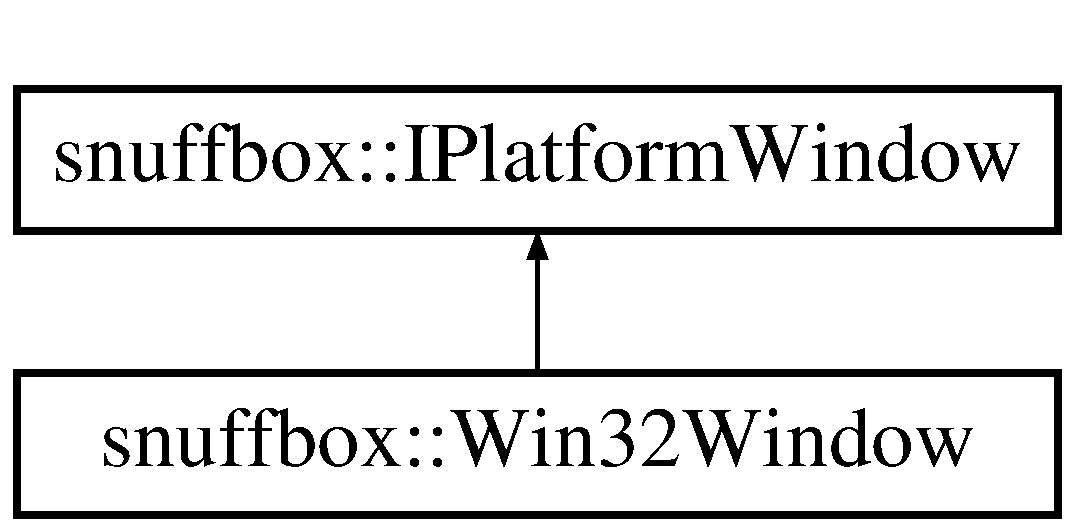
\includegraphics[height=2.000000cm]{classsnuffbox_1_1_win32_window}
\end{center}
\end{figure}
\subsection*{Public Member Functions}
\begin{DoxyCompactItemize}
\item 
\hypertarget{classsnuffbox_1_1_win32_window_aa294cac178581af0fe71c98ac6de8d9e}{\hyperlink{classsnuffbox_1_1_win32_window_aa294cac178581af0fe71c98ac6de8d9e}{Win32\-Window} ()}\label{classsnuffbox_1_1_win32_window_aa294cac178581af0fe71c98ac6de8d9e}

\begin{DoxyCompactList}\small\item\em Default constructor. \end{DoxyCompactList}\item 
\hyperlink{classsnuffbox_1_1_win32_window_a734120d1db7e699eb2df74ab70af8d9c}{Win32\-Window} (const char $\ast$name, int w, int h, int x=S\-N\-U\-F\-F\-\_\-\-W\-I\-N\-D\-O\-W\-\_\-\-C\-E\-N\-T\-E\-R\-E\-D, int y=S\-N\-U\-F\-F\-\_\-\-W\-I\-N\-D\-O\-W\-\_\-\-C\-E\-N\-T\-E\-R\-E\-D)
\begin{DoxyCompactList}\small\item\em Constructs a window with a width, height and position. \end{DoxyCompactList}\item 
\hypertarget{classsnuffbox_1_1_win32_window_ab7712ac2a0d08d2b9a6a617ea3c4bebf}{\hyperlink{classsnuffbox_1_1_win32_window_ab7712ac2a0d08d2b9a6a617ea3c4bebf}{$\sim$\-Win32\-Window} ()}\label{classsnuffbox_1_1_win32_window_ab7712ac2a0d08d2b9a6a617ea3c4bebf}

\begin{DoxyCompactList}\small\item\em Default destructor. \end{DoxyCompactList}\item 
\hypertarget{classsnuffbox_1_1_win32_window_abb9e8f647edcea6ba27106e957669879}{void \hyperlink{classsnuffbox_1_1_win32_window_abb9e8f647edcea6ba27106e957669879}{Create} ()}\label{classsnuffbox_1_1_win32_window_abb9e8f647edcea6ba27106e957669879}

\begin{DoxyCompactList}\small\item\em Creates the window. \end{DoxyCompactList}\item 
\hypertarget{classsnuffbox_1_1_win32_window_a9b691d7bc96d62cab570e25b12304ced}{void \hyperlink{classsnuffbox_1_1_win32_window_a9b691d7bc96d62cab570e25b12304ced}{Show} ()}\label{classsnuffbox_1_1_win32_window_a9b691d7bc96d62cab570e25b12304ced}

\begin{DoxyCompactList}\small\item\em Shows the window. \end{DoxyCompactList}\item 
\hypertarget{classsnuffbox_1_1_win32_window_aa62da0a61e669e341ac6eae45572c758}{void \hyperlink{classsnuffbox_1_1_win32_window_aa62da0a61e669e341ac6eae45572c758}{Destroy} ()}\label{classsnuffbox_1_1_win32_window_aa62da0a61e669e341ac6eae45572c758}

\begin{DoxyCompactList}\small\item\em Destroys the window. \end{DoxyCompactList}\item 
\hypertarget{classsnuffbox_1_1_win32_window_a9f69386a12a6ee5c2d1f8d7bf354ed65}{void \hyperlink{classsnuffbox_1_1_win32_window_a9f69386a12a6ee5c2d1f8d7bf354ed65}{On\-Set\-Focus} ()}\label{classsnuffbox_1_1_win32_window_a9f69386a12a6ee5c2d1f8d7bf354ed65}

\begin{DoxyCompactList}\small\item\em When the window is focussed. \end{DoxyCompactList}\item 
\hypertarget{classsnuffbox_1_1_win32_window_a80cd30171c96ad76001392c7a816631a}{void \hyperlink{classsnuffbox_1_1_win32_window_a80cd30171c96ad76001392c7a816631a}{On\-Kill\-Focus} ()}\label{classsnuffbox_1_1_win32_window_a80cd30171c96ad76001392c7a816631a}

\begin{DoxyCompactList}\small\item\em When the window focus is killed. \end{DoxyCompactList}\item 
\hypertarget{classsnuffbox_1_1_win32_window_abcf0d96e1c607d9613fa99a5bd3bbfd0}{void \hyperlink{classsnuffbox_1_1_win32_window_abcf0d96e1c607d9613fa99a5bd3bbfd0}{On\-Close} ()}\label{classsnuffbox_1_1_win32_window_abcf0d96e1c607d9613fa99a5bd3bbfd0}

\begin{DoxyCompactList}\small\item\em When the window is closed. \end{DoxyCompactList}\item 
\hypertarget{classsnuffbox_1_1_win32_window_a46f23dcc30eb823ee06599eae5e3824d}{void \hyperlink{classsnuffbox_1_1_win32_window_a46f23dcc30eb823ee06599eae5e3824d}{Process\-Messages} ()}\label{classsnuffbox_1_1_win32_window_a46f23dcc30eb823ee06599eae5e3824d}

\begin{DoxyCompactList}\small\item\em Processes all messages. \end{DoxyCompactList}\end{DoxyCompactItemize}


\subsection{Detailed Description}
A Windows window for use with the engine. 

\begin{DoxyAuthor}{Author}
Dani�l Konings 
\end{DoxyAuthor}


\subsection{Constructor \& Destructor Documentation}
\hypertarget{classsnuffbox_1_1_win32_window_a734120d1db7e699eb2df74ab70af8d9c}{\index{snuffbox\-::\-Win32\-Window@{snuffbox\-::\-Win32\-Window}!Win32\-Window@{Win32\-Window}}
\index{Win32\-Window@{Win32\-Window}!snuffbox::Win32Window@{snuffbox\-::\-Win32\-Window}}
\subsubsection[{Win32\-Window}]{\setlength{\rightskip}{0pt plus 5cm}snuffbox\-::\-Win32\-Window\-::\-Win32\-Window (
\begin{DoxyParamCaption}
\item[{const char $\ast$}]{name, }
\item[{int}]{w, }
\item[{int}]{h, }
\item[{int}]{x = {\ttfamily SNUFF\-\_\-WINDOW\-\_\-CENTERED}, }
\item[{int}]{y = {\ttfamily SNUFF\-\_\-WINDOW\-\_\-CENTERED}}
\end{DoxyParamCaption}
)}}\label{classsnuffbox_1_1_win32_window_a734120d1db7e699eb2df74ab70af8d9c}


Constructs a window with a width, height and position. 


\begin{DoxyParams}[1]{Parameters}
\mbox{\tt in}  & {\em name} & (const char$\ast$) The name of the window \\
\hline
\mbox{\tt in}  & {\em w} & (int) The width of the window \\
\hline
\mbox{\tt in}  & {\em h} & (int) The height of the window \\
\hline
\mbox{\tt in}  & {\em x} & (int) The x position of the window (optional, will center if left out) \\
\hline
\mbox{\tt in}  & {\em y} & (int) The y position of the window (optional, will center if left out) \\
\hline
\end{DoxyParams}


The documentation for this class was generated from the following files\-:\begin{DoxyCompactItemize}
\item 
C\-:/\-Snuff/src/snuffbox/win32/win32\-\_\-window.\-h\item 
C\-:/\-Snuff/src/snuffbox/win32/win32\-\_\-window.\-cc\end{DoxyCompactItemize}

%--- End generated contents ---

% Index
\newpage
\phantomsection
\addcontentsline{toc}{chapter}{Index}
\printindex

\end{document}
